

\chapter{Online Hyperbolic Latency Graph Embedding as Synthetic Coordinates for Latency Reduction in Distributed Hash Tables}
%
%
% author names and IEEE memberships
% note positions of commas and nonbreaking spaces ( ~ ) LaTeX will not break
% a structure at a ~ so this keeps an author's name from being broken across
% two lines.
% use \thanks{} to gain access to the first footnote area
% a separate \thanks must be used for each paragraph as LaTeX2e's \thanks
% was not built to handle multiple paragraphs
%
\begin{center}
Brendan~Benshoof, Andrew~Rosen, Dr.~Robert~Harrison
\end{center}



\section{Introduction}

There is an inherent trade-off between availability and latency minimization in DHT design. 
A design that always ensures minimal latency routes is a clique\cite{li2013zht} which requires 1 hop for lookups.

However this design requires all members of the network to maintain $O(n)$ connections, which limits the scalability of such a system.

Distributed Hash Tables seek to ensure the scalability of the system by requiring nodes to track only $O(\log{n})$ nodes in the network, which necessitates higher latency in queries over the Distributed Hash Table.
We present a technique to minimize the maintenance overhead and query latencies within the constraint of maintaining the scalability of the network.

Distributed Hash Tables form the core of many P2P systems like Bitorrent\cite{jimenez2011kademlia}, CJDNS\cite{hodson2013meshnet}, and I2P\cite{zantout2011i2p}.
Increasing the response time and efficiency of DHTs will provide these systems and systems like them with increased performance and capacity to scale to more users.

\section{Background}

The ideas applied in this paper pull from a variety of backgrounds, including wireless networking, graph embedding and hyperbolic geometry.

\subsection{Geographic Routing}

Geographic routing is used in CDN latency optimization and Wireless Sensor Networks\cite{karp2000geographic}.
The basic premise, is unlike traditional network routing mechanism, messages can be routed in a network based on the location of the current node and the location of the destination.
While the ideal is that messages could be routed greedily, the realities of radio and connectivity limitations have resulted in a number of proposed algorithms.

There are serious concerns with application of simple geographic routing in practice.
Geographic locations may not accurately represent network connectivity and latency.
Often holes" or "lakes" in the network prevent greedy routing, requiring more complex and stateful routing methods to act as auxiliary to greedy routing.
The fundamental problem being that due to the inability to make connection past an obstacle 

While we will take inspiration from the mechanisms of greedy geographic routing, distributed hash tables are not vulnerable to the problem of untraversable terrain that plagues wireless sensor networks. 
So while in practice, so long as a greedily traversable graph is maintained, we can use only the greedy geographic forwarding strategy to route messages.
This leaves us with the problem that locations and routes in space often do not match the throughput and latency reality of the network.
The focus of this work is building a coordinate system alternative to geographic location that provides the capacity to leverage greedy geographic routing for both successful and efficient routes.

\subsection{Greedily Traversable Mesh}

The idea of a greedy traversable Mesh is that based on a distance estimator, a route can be found between between any two nodes by greedy best first search without any backtracking.

This provides efficient routing through the network without maintaining any state in the packet or maintaining routing tables.

\subsubsection{DGVH}

DGVH\cite{dgvh} is a technique for building minimal greedy traversable meshes in arbitrary metric spaces (it requires that distances follow the triangle inequality and are symmetric between 2 points)

algorithm for peer selection:
\begin{enumerate}
	\item Given a $center$ node we are finding the Peer List for
	\item Initialize a empty $Peers$ list
	\item Consider the list $Candidates$ of candidate peers sorted by increasing distance from $center$
	\item Pop the closest member of $Candidates$ and add it to the $Peers$ list. $center$ will always peer with the closest node to it.
	\item For the remaining nodes $c$ in $Candiates$
	\begin{enumerate}
		\item if $c$ is closer to $center$ than any current members of $Peers$ then add it to the $Peers$ list
		\item else discard $c$
	\end{enumerate}
\end{enumerate}





\subsection{Scale Free Networks}

Scale free networks are a family of tree-like networks defined by an having expoential  degree distribution, and a tendency for high-degree nodes to be linked to other high degree nodes.

These properties describe a network with a $O(\log{n})$ diameter, which in practical systems can often be considered constant.

Scale free Networks are of interest to us because they are a generalization of the connectivity topology of human build digital networks.
The latency distribution of a representative sample of computer in the global internet should show a latency similar to that of a representative subset of a scale free graph.


\section{Previous Works}

\subsection{Kleinberg's Hyperbolic Embedding}
A distributed and dynamic hyperbolic embedding of latency suitable for optimizing a distributed hash table was envisioned by Robert Kleinberg in 2007.

\subsubsection{Greedy Embedding}
The Greedy Embedding discussed by Kleinberg is inverse to the "DGVH" method of generating a greedy traversable mesh discussed above.
Rather than being given a set of points and generating a traversal mesh, we are given a graph and solve for points for each node such that resulting mesh is greedy traversable.

Initially discussed Papadimitriou et al\cite{papadimitriou2004conjecture} by A greedy embedding can be formally defined as a distance function between two points $d(a,b)$ in a given metric space and a transformation $f(v)$ that maps each vertex in the given graph such that for every pair of non-adjacent vertices $a,v\in G$ there exists a third vertex $c$ adjacent to a such that $d(u,b) < d(a,b)$. 
Essentially, the result of this definition is that for any vertices not directly connected, there exists a path of nodes that iterativly closer to the target that could be followed by greedy traversal (interestingly, graphs produced by DGVH are forced by the algorithm to fulfill this property making it an inverse function to greedy embedding)

\subsubsection{Life on the Hyperbolic Plane}
Hyperbolic space in 2 dimensions is defined as the surface of a hyperbola in 3 dimensions where all paths between points are taken along the surface of the hyperbola.
This hyperbola is defined by the equation $z^{2}=x^{2}+y^{2}+1$.
Note that for any $(x,y)$ pair there exists 2 solutions for the value of $z$, one positive and the other negative.
These two solutions form 2 disconnected "sheets" mirrored across the xy-plane.
By convention we only consider points on the negative z sheet (all calculations and processes work effectively on either sheet as long as all considered points are on the same sheet).

The hyperbolic plane has many differing qualities from the euclidean plane, most importantly is that of "relativity".
On a euclidean plane, we can treat any point as the "origin" and calculate new locations for every point or figure on that plane by translation, and have all inter-point angles and distances remain the same.
The euclidean distance equation $\sqrt{(x_{1}-x_{0})^{2})+(y_{1}-y_{0})^{2})}$ can be interpreted as translating $(x_{1},y_{1})$ into the reference frame where $(x_{1},y_{1})$ is the center, and using the distance metric $\sqrt{x^{2}+y^{2}}$ to determine the distance.
Unlike this, the hyperbolic plane has a defined center, and while points can be rotated and mirrored freely over this center without changing inter-point distance and angle, they cannot be translated.
The distance between two points in the hyperboloid model is $\operatorname{arcosh}(z_{0}z_{1} - x_{0}x_{1} - y_{0}y_{1})$ where $\operatorname{arcosh}x$ is defined as $\ln{(x+\sqrt{x^{2}+1})}$

Unlike euclidean space, a 2d Hyperbolic Plane has a Greedy Embedding for any graph.
Kleinberg presents his technique for building arbitrary graph embedding in hyperbolic spaces by building a spanning tree of the graph, then embedding the tree into the hyperbolic space.
This is effective because the circumference of the disk increases exponentially with radius, therefore we can trivially embed trees into the space as the available space on the disk increases in correspondence with the number of leaves in a full tree.
While greedily traversable, the resulting embedding does not provide desirable qualities in that greedy routes are not necessarily the shortest and central nodes receive high levels on congestion.



\subsection{Greedy Hyperbolic Embedding}
Further work by Papadopoulos et al\cite{papadopoulos2010greedy} shows an greedy centralized technique for managing the creation of a dynamic network in a hyperbolic space.
Papadopoulos presents improvements over Kleinberg's initial work by presenting a simple stratagy for handling node joining the network (greedy insertion) to minimize path latency and routing methods to handle node and edge failure.



\subsubsection{Growing Network with Greedy Embedding}

Papadopoulos et al provide a sophisticated method for accurate generating a growing scale free network in a hyperbolic space. It is important to note that they are creating a new topology and network from scratch, rather than attempting to use existing latency information to build a Greedy Embedding that also represent that network topology.

Papadopoulos et al show that graphs with similar properties to those found in the "nature" of real world network topologies can be generated and have desirable greedy routing properties.
This is accomplished by randomly selecting points in the hyperbolic space such that, all points are constrained within a given disk that represents the network radius and a distribution of radius that represents the branching factor of the scale free graph intended to be simulated.

Points are then connected together randomly, using a model weighted by inter-node distance and angle.

\subsubsection{Utility in building a Hyperbolic DHT}

While interesting, the statistical method of peer selection proposed is insufficent for ensuring a Greedy Embedding that can be navigated under churn. The proposed Gravity-Pressure routing method requires packets maintain an nonviable amount of state information without reasonable benefit.
It begins to follow the path of geographic routing techniques with growing sophistication in response to an environment that is not greedy routable.
We are better served by ensuring the environment it greedy routable than attempting to add overhead to routing to manage failures of topology maintenance.




\section{Contribution}


We present a technique for building a Distributed Hash Table on a hyperbolic metric space to minimize  look-up and maintenance latency within the constrains of ensuring the scalability of the system.
We show a simple greedy method for inserting nodes into the network such that latency is congruent 
with the distance metric.
We show that unlike previous works indicate, no special updating of node location is required in response to the joining or exiting of new nodes and in fact a constant churn rate will help the system respond to changes in global latency distribution.
We have found that if we augment the network topology with a greedy navigable mesh, holes introduced via node loss are accurately repaired and new nodes are greedily inserted at latency ideal locations in the network.

\subsection{The Value of Approximation}
Unlike previous work, in presenting a practical DHT description, we are dealign with different premises than previous work with hyperbolic embedding.
The largest divergence from Kleinberg and Papadopoulos works is that rather than dealing with embedding a scale free graph, we are embedding a effectivly random sampling of a massive scale free graph in the form of the internet.
Secondly, we will be dealing with constant churn of members of the network, and changes in inter-node latnecy over time.
The consequence of this is that the exact methods proposed in previous work, which promise essentially optimial routes cannot be extended into reality in that fashion.
Because we are dealing with a sampling of a scale free graph, rather than the entire graph, we will induce stetch simply because we cannot connect all nodes in the overlay network as a clique. 
We are bound to the scalaibility limitations of a distributed hash table.


\subsection{Hyperbolic DHT Model}

We establish an Hyperbolic DHT Network in the hyperbolic plane using the hyperboloid model. While any hyperbolic plane representation will work effectively, for accurate internal representation we utilize the x,y,z coordinates of points in the 3d hyperbolic sheet rather than poincare disk or similar representations due to the inability of floating point numbers to accurately represent values at the extremes of those models.

%describe the hyperboloid model in detail?

Using a direct application of DGVH's capacity to build greedy traversable overlay networks in arbitrary metric spaces, we can extend the contrived metric spaces of Chord and Kademlia into a more general model. This would allow DHTs to be constructed in any metric with the triangle inequality and symmetric distance. Conveniently, as it is the focus of this paper, the hyperbolic plane metric space is easy for DGVH to utilize.

We will use points on the hyperbolic plane in the hyperboloid representation\cite{jansen1909abbildung} (3d coordinates of points on the bottom sheet of the hyperbola) with the distance metric $\operatorname{arcosh} (z_{0} \cdot z_{1} - x_{0} \cdot x_{1} - y_{0} \cdot y_{1})$

\subsubsection{Joining and Embedding}

The only divergence from a traditional DHT's operation is in the assignment of points in the coordinate space to joining nodes.
To preserve the accuracy of the embedding, we must place nodes in the network at a point where they have low local latency.
Given that the goal of the embedding is that paths can be routed with minimal latency, the leverage the inverse to greedily place nodes into the network.

Given any arbitrary node in the network as a start point, the joining has two sequential greedy searches:

First the joining node greedily searches for the location <0,0,-1> which represents the "center" of the network.
Once we have a reference to a node at the center of the network the preform a greedy best first search similar to before, but rather than looking up the next hop, we query a node for its peers. We then ping each peer to test latency. We select the peer with lowest latency and iterate this process until we have found a node to which we have lower latency than all of its peers. We select a location subordinate to this node and preform a traditional UrDHT join at this location.


\begin{enumerate}
	\item build a greedy navigable mesh over points in the hyperbolic embedding to augment routing and ensure delivery using greedy forwarding under churn
	\item describe a greedy algorithm for joining nodes to discover ideal insertion points starting from any node in the network
\end{enumerate}

\subsection{Routing and Message Passing in the Hyperbolic DHT}
Routing uses a modified "recursive" method.

It is important to note that usage of the overlay network does not provide any increase in efficiency, rather it provides an efficient mechanism for finding the owner of a given location with minimal overhead while preserving the capacity of the network to scale to arbitrary size efficiently. 

A message has a destination location in the hyperbolic space, query message and callback IP and port to return the response to.
Generally a message will be targeted to a specific location in the metric space, rather than a specific server, and whichever server is responsible for that location will handle the query.
Often a message will originate from a user who is not even a member of the DHT querying to store a value or retrieve a stored value.

A message will begin in the network at a selected "sponsor", who hopefully is chosen for low latency with the user, but this is not required and a sponsor can simply be any known member of the DHT.
The message is passed between members of the DHT using a greedy "best first" strategy, that forwards the message to the peer closest to the destination location (in this case using the distance along the geodesic).
No trace-back or hop count information is required to ensure delivery, and a node will consider itself the destination of the message when it is closer to the destination location than any of its peers.
Once the query message is handled (often storing or retrieving a value), the response (a success notification or the requested data) will be sent directly to the user rather than using the overlay network.


\subsection{Storing Records on the Hyperbolic Surface}

The traditional mechanism of mapping keys to cryptographic hashes is less intuitive when locations in the space are actual points rather than integers.
The most straightforward method is to design a pseudo-random point generator, that can be seeded using the more traditional cryptographic hash.
Care must be taken to ensure that the results of this process are evenly distributed.
Using a classical pseudo-random number generator like mersenne-twister with classical 32-bit or 64-bit data types will bound the maximum number of unique locations to the number of unique integers the PRNG can generate, and as the distributed system grows in size increases to the size and format of these identifiers may be required.

As we are using the Hyperboloid model of representing points in hyperbolic plane, we must map our hash values onto the hyperbolic plane with the goals of distributing those point evenly in portions of the plane actually occupied by nodes in the system.
Given a centered and bounded disk on the hyperbolic plane in which all nodes fall, we can expect the distribution of nodes to be linear over the polar angle an exponentially distributed over the radius. 


Using the following algorithm to produce points will evenly distribute the random points over the disk up to MAXRADIUS. A maximum radius is required because a higher share of points will be distributed to locations distant from the origin of the space as the circumference of the space increases exponentially in response to radius. While it would be possible to distribute points over an unbounded space statistically, in this case the majority of points would be assigned to portions of the hyperbolic disk increasingly distant from the embedding of the DHT nodes.  
\begin{enumerate}
	\item SEED(HASH(key))
	\item ANGLE = $2\pi{} \dot{} \mathit{RANDOM()}$
	\item RADIUS = $\mathit{MAXRADIUS} + \frac{\log{(1-{\mathit{RANDOM()}})}}{\mathit{MAXRADIUS}}$
\end{enumerate}


While it is perfectly possible that the network would either be smaller or larger in radius than a pre-chosen MAXRADIUS, the disparity in load due to this is likely a preferable problem then attempting to vary MAXRADIUS at runtime. (If there is an expectation of the network's size at the time of establishment, an appropriate MAXRADIUS can be chosen in respect to that.

No matter what MAXRADIUS is chosen, all keys will be assigned to responsible nodes, however if MAXRADIUS is smaller than the network radius then it is likely nodes on the periphery will not be assigned records (this may be ideal behavior in more general systems than a DHT, as these nodes will likely have high latency)

\section{Analysis}

\subsection{Network Diameter}

We present two independent arguments that the diameter of a greedy traversable graph embedding of a scale-free graph in the hyperbolic plane is $O(\log{n})$

Given that the diameter of a scale free graph is $O(\frac{\log{n}}{\log{\log{n}}})$\cite{bollobas2004diameter} and the greedy embedding is a super-set of this graph (and being a super-set could only reduce the diameter) the diameter of the embedding is $O(\frac{\log{n}}{\log{\log{n}}})$ or better which falls in $O(\log{n})$

Given that the greedy insertion algorithm attempts to uniformly insert nodes into a bounded hyperbolic plane such that the Voronoi regions of these nodes are approximately equal in area.
Area of the hyperbolic disk is effectively a exponential function of the radius, thus the average shortest path in the network is expected to cross $O(\log{n})$ regions.

\subsection{Expected Path Stretch}

The ideal stretch ratio ($\frac{\mathit{Actual Path Length}}{\mathit{Optimal Path Length}}$) for the hyperbolic embedding is $O(1))$.
This stretch is caused by errors in the embedding taking non-optimal routes.
Previous works show that greedy routing in the hyperbolic overlay are $O(1)$
Even if the accuracy of the hyperbolic embedding fails due to unforeseen technical problems or active attack, the properties of the hyperbolic space ensure that the stretch factor is no worse than if nodes were connected randomly as in a traditional DHT.

The stretch ratio observed in existing DHTs is the number of hops required to complete a lookup.
In practice, the distance between any successive hops in the lookup is expected to be the average inter-node distance, thus the expected stretch is $O(\log{n})$ times the average inter-node distance. 

\begin{figure}[H]
	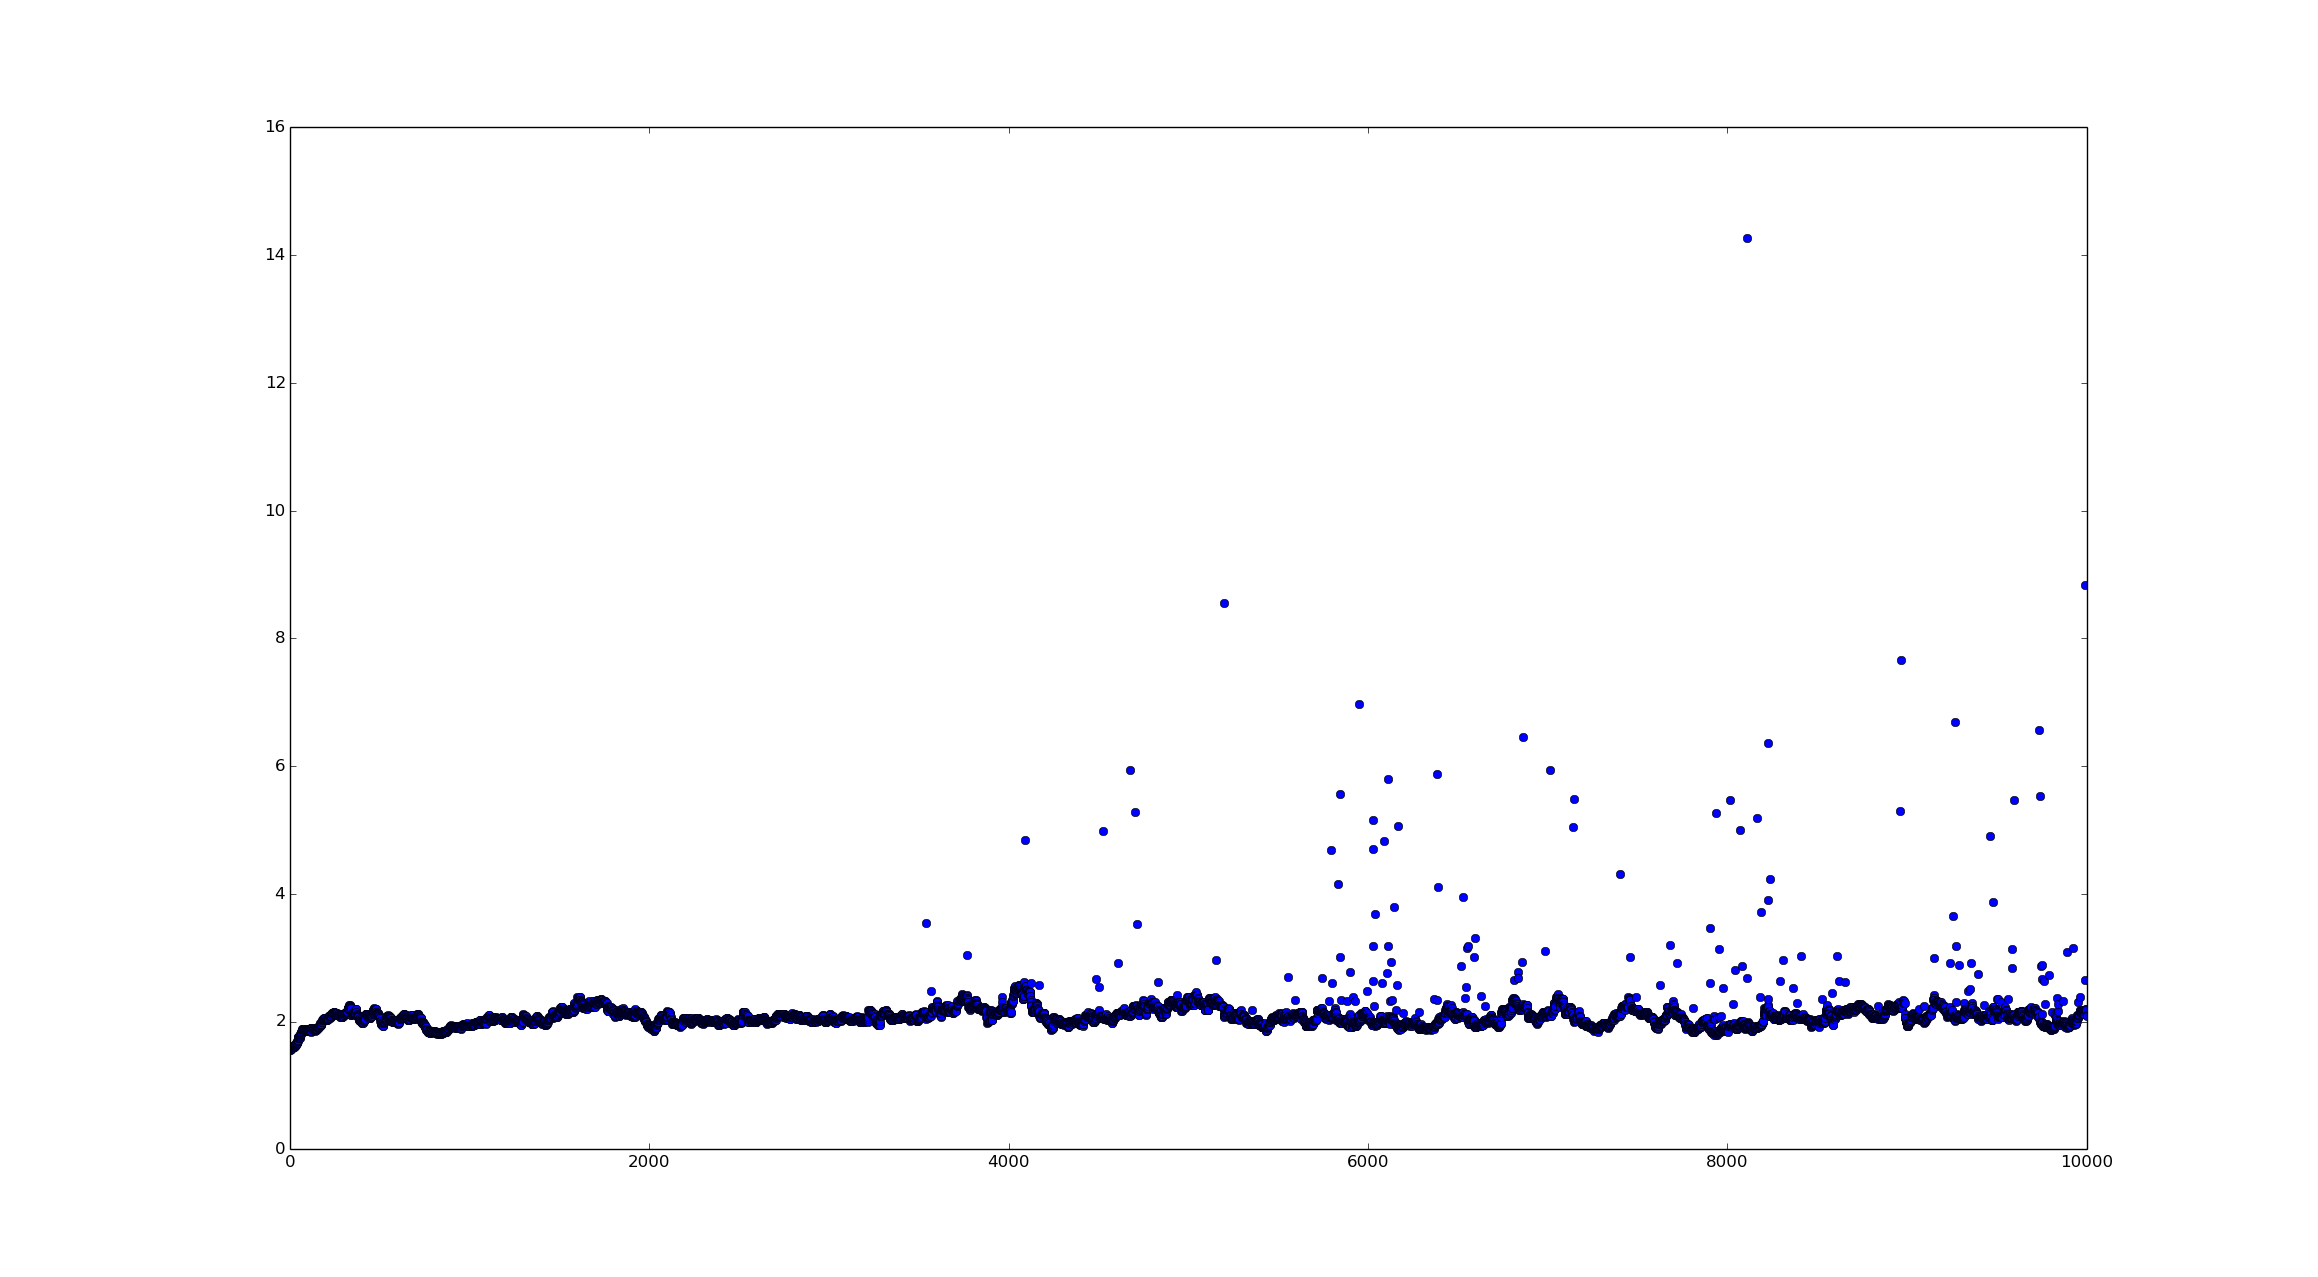
\includegraphics[width=\textwidth]{churn_stretch}
	\caption{Here we see the stretch factor (essentially embedding quality) over time as nodes exit and join the network. Removal of central nodes can often require a short period of re-ajdustment, but stretch maintains stablility over time}
\end{figure}


\subsection{Congestion and Route Diversity}
Problematically, the maintenance latency and lookup latency provided by hyperbolic embedding have an inherent disadvantage noted by previous authorities on the topic\cite{kleinberg2007geographic}. 
This latency reduction comes from having the connectivity of the distributed hash table congruent to the connectivity of the underlying scale free graph.
The degree distribution and low number of central nodes in a scale free graph forces most routing paths through high degree central nodes.

While we cannot easily decrease the maintenance overhead due to high degree, we can manage congestion using a simple mechanism.
Because DGVH maintains a list of long peers, (a size limited subset of all the "short-peers" of my "short-peers") every node connected to a central node, has a random sampling of "short-cuts" across the network that bypass high centrality nodes.
Only when the "long peers" fail to provide a reasonable alternative is a message routed to a higher centrality node.
While this dramatically reduces the network throughput required for central nodes, it should still be expected that central nodes will have a higher throughput requirement then those on the periphery of the network, but less so than the concerns of previous works\cite{kleinberg2007geographic}.
This also points out that for future work, in general, reducing the diameter of the network reduces the overall work the system has to do, and building "short cuts" around high degree nodes reduces the concentration of congestion around central nodes in a concept parallel to Kleinberg's small world networks\cite{kleinberg2000navigation}

Additional congestion avoidance behavior is trivial to implement because the DGVH mesh greedy routing can effectively route around holes, when a node is reaching congestion saturation, it can begin to respond to routing queries with a failure message, causing the forwarding algorithm to bypass the overloaded node, if the overloaded node is the only viable path to the destination, then the resulting loop the packets follow will act as an ad-hoc buffer, storing and re-trying sending messages to congested peers until they can be accepted, effectively using the network as a memory in much the same sense as a mercury delay line\cite{auerbach1949mercury}.

\begin{figure}
	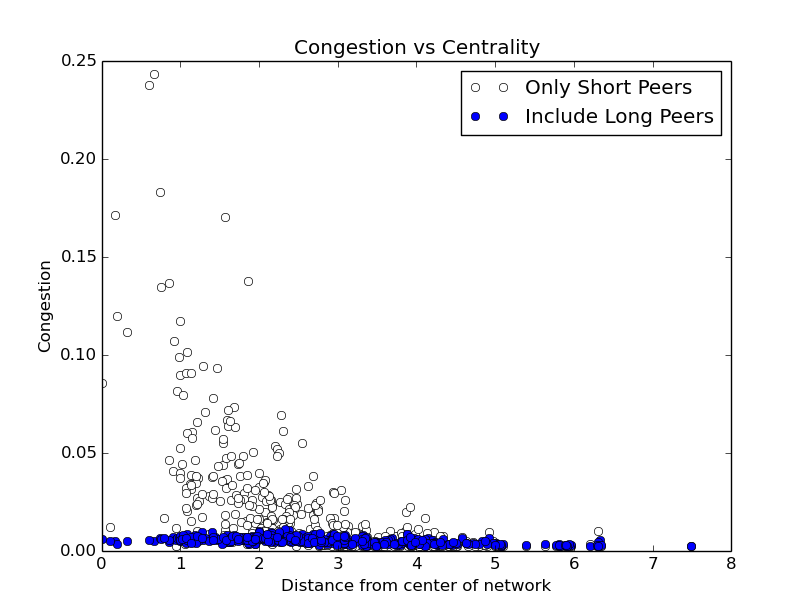
\includegraphics[width=0.5\textwidth]{radius_vs_load}
	\caption{Here we see the congestion when using short peers only (approximating a scale free graph) and when utilizing randomly selected long peers.
		Using only short peers shows that central nodes handle disproportionate amounts of messages.
	}
\end{figure}

\begin{figure}
	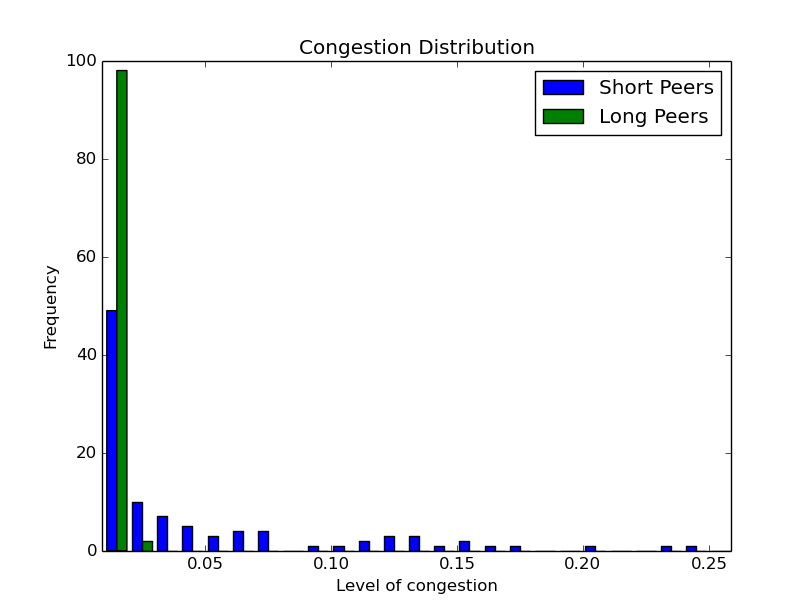
\includegraphics[width=0.5\textwidth]{congestion_4}
	\caption{Using only short peers forces more nodes, to take on higher congestion versus using long peers which globally reduces congestion.
	}
\end{figure}

\subsection{Simulation}

We simulate the greedy construction of a hyperbolic embedding and show that they produce very low latency stretch

\begin{figure}
	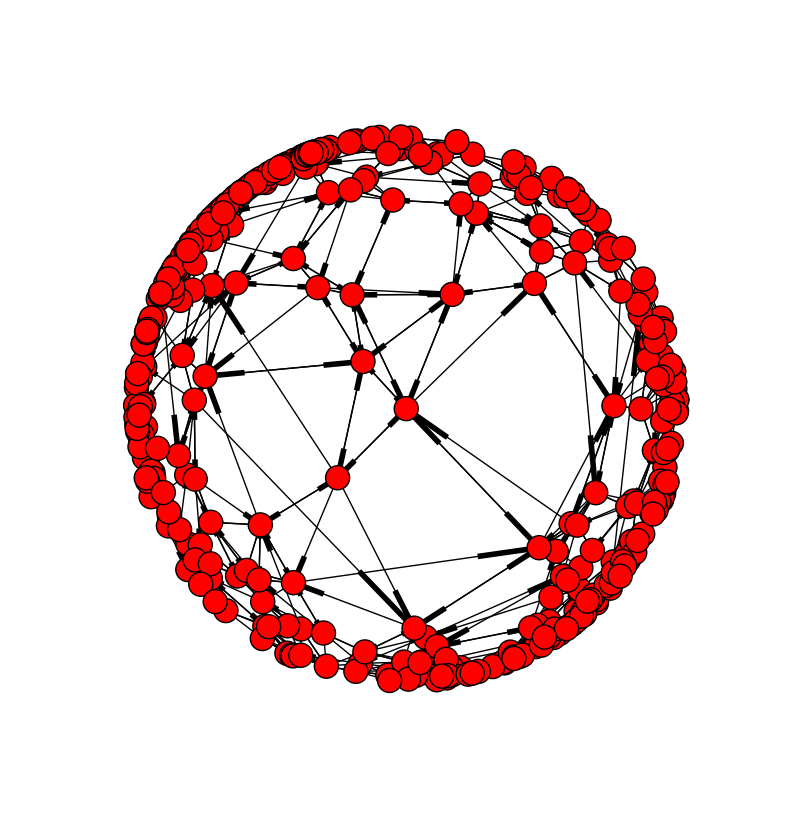
\includegraphics[width=0.5\textwidth]{disk}
	\caption{
		This is an example of the short-peer topology of a network embedded into hyperbolic space viewed through the Poincaré Disk model.
	}
\end{figure}


We simulate churn in a dynamic embedding and show that the embedding retains low latency stretch over time. We generate a 1000 node scale free graph and a size 100 overlay DHT. For 10,000 iterations we randomly select a node from the overlay and remove it, and then randomly select a node from the 1000 node underlay network and greedily insert it into the network using the join method discussed above then record and log the average route stretch.

The resulting network though churn has been totally replaced many times during the process of the simulations. 
While the quality of the simulation degrades initially from a stretch factor of 1.7, the stretch factor fluctuates around 2.0 as the simulation progresses.
Showing that greedy insertion is effective and maintaining the embedding under churn.


\section{Conclusions}
We show that a decentralized algorithm for embedding overlay networks is possible by building a greedy traversable mesh to augment a greedy embedding.
This approach is possible because we work under different assumptions than previous work, as we are attempting to approximately embed a subset of a very large scale free graph rather than a perfect embedding of an entire scale free graph.
We have shown that stretch over optimal latency is O(1) and that a finite amount of long peers can dramatically reduce network congestion and disproportionate query load in the network.

\subsubsection{Concerns and Future Work}

While we consider application of this system to practice a straightforward practice extending previous work in DGVH\cite{dgvh} usage in real systems presents a new issue.
While previous DHTs could be "optimized" to reduce effort by storing replicas of stored data at points adjacent to the host, because adjacent peers in the hyperbolic overlay are more likely to be physically close to one another, the statistical assurances provided by such robustness mechanism are weaker and such strategies should be re-examined before implementing a system similar to the one proposed in this work.






